\documentclass[journal, a4paper, twoside, romanappendices]{IEEEtran}
% !TEX root = ./report.tex

\usepackage{datetime}	%For \newdateformat
\usepackage{float}		%For forcing position of figures
\usepackage{listings}	%For code in document
\usepackage[usenames,dvipsnames]{color}	%For the SkyBlue background color for lstlistings
\usepackage{todonotes}	%For \todo
\usepackage{tabularx}	%for tablecontents wrapping inside cell, instead of cell breaking page width.
\usepackage{enumerate}	%For getting different types of lists like a) II) and so forth.
\usepackage[utf8, utf8x]{inputenc}	%For norwegian letters and UTF8 encoding support
\usepackage{lastpage}	%For the command \pageref{lastpage}
\usepackage{hyperref}	%For \url{}

\newdateformat{CurMonth}{\monthname[\THEMONTH],~\THEYEAR}


\begin{document}

\title{When should one inline recursive functions?}
\author{Christian~Chavez}
\maketitle

\thanks{Nico~Reissmann, Magnus~Jahre, and Christian~Chavez are with the
Norwegian University of Science and Technology (NTNU).}


\begin{IEEEkeywords}
Function inlining, Jive, Compiler, 2015, NTNU
\end{IEEEkeywords}

% !TEX root = ./report.tex

\begin{abstract}

\blindtext

\end{abstract}

%% !TEX root = ./stuff.tex

\todo[inline]{Figure out the terms found in papers...}

\section{\cite{GHCPaper}}
\begin{enumerate}

	\item Section 1
\begin{itemize}

	\item ``inlining subsumes''
Something gets removed by inlining.

	\item ``lexical scopes''
Scope of a program/function/block/variable.
From StackOverflow:
\url{http://stackoverflow.com/questions/1047454/what-is-lexical-scope}

	\item ``pure'' (\textit{language})
Program must always return same results with same inputs. There can be no
``side-effect'' which changes the state of the program.

	\item ``explicitly typed'' (\textit{language})
That the compiler knows at compile time (static) what types all the variables
and return values have.
Great explanation: \url{http://programmers.stackexchange.com/questions/181154/type-systems-nominal-vs-structural-explicit-vs-implicit}

	\item ``strictness analysis''
\todo[inline]{Need more research}
\url{http://en.wikipedia.org/wiki/Strictness_analysis}
\url{https://ghc.haskell.org/trac/ghc/wiki/Commentary/Compiler/Demand}

	\item ``\textit{let}-floating'' (\textit{Haskell})
Nico: Not important.

	\item ``name capture''
Making sure each name is an unique identifier. This gets complicated when
compiler has to rename things for program correctness. Like when inlining.

\end{itemize}

	\item Section 2
\begin{itemize}

	\item ``\textit{$\beta$}-reduction''
A way of utilizing lambda-calculus to simplify a lambda expression. Closely related to simplifying anonymous functions (lambda functions) in pure functional programming languages like Haskell.

	\item ``invariant'' (\textit{language artifact/variable/expression?})
Constant/Unchanging: Unchanged by mathematical or physical operations or
transformations.

	\item ``\textit{trivial-constructor-argument invariant}'' (\textit{Haskell?
})
See directly above.

	\item ``divergent computations''

	\item ``closure'' (\textit{scopes of functions?})
Ensuring correct lexical scope for (free)variables, mainly needed in languages
permitting nested function.

	\item ``lambda calculus''
An important language, focusing on ``\textit{computational mathematics}''. It is
\textit{Turing complete}, and it can represent any program. As mentioned, it
focuses on the computational operations of a ($\lambda$-)function, unlike
``normal functions'' which focus on their respective inputs and outputs.

	\item ``literals''
The string ``abcd'' is a literal. As is the number 1, when used to assign value
to an integer, just like the string is used to assign value to a string-variable.

	\item ``primitive operators''
Operators that are in one way ``basic'', but not necessarily only (nor all) of
the operations supported by hardware. Think of it as the most basic operators
which together build up all others.

\end{itemize}

	\item Section 3
\begin{itemize}

	\item ``bound variable''
A variable that is not free, that is, a variable which has been specified as an
input to a function call. (The opposite of a free variable, which is a variable
used in a function, but declared outside of it, and not listed as one of its
parameters).

	\item ``recursive binding groups''
When you have calls between groups of recursive functions, complicated
situations arise. See \cite{GHCPaper}, Section 3.5 for example of a ``recursive
binding group''.

	\item ``strongly-connected components''
A group of nodes (\textit{components}) in a DAG where you can reach every other
node/component/vertex from any other. Hence, a DAG might have several \textit
{strongly-connected components}, composed of a multiple of
nodes/vertices/components.

	\item ``contravariantly''
	(\textit{(..) it appears contravariantly in its own definition.})
Best guess: This term refers to variables or functions which are declared, and then used in a manner contradicting the nature of their declaration. Which possibly can become a problem when inlining recursive functions.

	\item ``untyped programs''
Nico: Not relevant.

	\item ``pathological programs''
Forgot, ask Nico again.

	\item ``static analysis''
Analysis at compile time.

\end{itemize}

	\item Section 4
\begin{itemize}

	\item ``hash-consing''

\end{itemize}

\end{enumerate}

% !TEX root = ./report.tex

\section{Introduction}
\label{introduction}

Since the 1950s, compilers have played an important role in the way programming
code is translated into machine languages. In broad terms, compilers perform two
actions: the translation from human-readable code to machine language, and
optimizing the translated programs. There exist many optimization techniques
compilers use. One such technique is inlining, where the call site of a function
is replaced by the body of the function, as shown in Listing \ref{lst:inlining}.

\begin{lstlisting}[label={lst:inlining}, style=customcpp,
caption={Function \textit{foo()} inlined into function \textit{bar()} would
result in the body of \textit{bar()} being \textit{return x + 3 + 2}, in which
case the optimization technique of constant folding is unveiled, permitting the
compiler to replace the expression with its cheaper equivalent: \textit{x +
5}.}]
int foo(int x){
	return x + 3;
}

int bar(int y){
	return foo(y) + 2;
}
\end{lstlisting}
\vspace{-4\parskip} %http://tex.stackexchange.com/q/40863

The benefits are manifold. Removal of function call overhead, and a potential
for unveiling the application of additional optimizations being among these. The
drawbacks is potential code-duplication, exemplified in Listing~\ref{lst:code-dup},
and in certain specific situations work-duplication\footnote{As detailed by P.
Jones and Marlow~\cite{GHCPaper} to be the case for the \textit{Glasgow Haskell
Compiler}.}. Another potential drawback is negatively affected compile time, and
increased program executable size.

\begin{lstlisting}[label={lst:code-dup}, style=customcpp,
caption={Code duplication in \textit{bar()}, when inlining \textit{foo()} into
\textit{bar()}. The big expression \textit{e} in \textit{foo()}, would be
duplicated when inlined into \textit{bar()}. This replaces the cost of function
call overhead with the increased size of the final program, unless potential
optimizations that counteract this are unveiled when inlining \textit{foo()}.}]
int foo(int a){
	return e; //Big expression, output of which depends on a's value
}

int bar(int x, int y){
	return f(x) + f(y);
}
\end{lstlisting}
\vspace{-4\parskip} %http://tex.stackexchange.com/q/40863

\todo[inline]{Consider removing: \\
Not all functions are straight-forward to inline, such as recursive functions.
At compile time, the needed depth of recursion might be unknown, leading to non-
termination of the compiler as it tried to inline the recursive function until
the necessary depth.}

This report describes the inliner project for the Jive compiler backend. It
details the decisions made for the inliner's architecture. Jive takes program
code in \textit{intermediate representation} (IR) as input and uses a new IR
representation, the \textit{Regionalized Value-State Dependence Graph}
(RVSDG\footnote{Detailed in Section \ref{background:RVSDG}.}).

\todo[inline]{Todo: In the below text (write it into the text) describe
layout/outline of paper. What does each section in turn discuss?}

The report will detail how the inliner is able to handle recursive functions,
and how the inliner permits the configuration of different heuristics to allow
rapid exploration of the parameter space. How the RVSDG affects the design of an
inliner, and the algorithms used by the heuristics deciding what to inline, is
also looked into in this report. Focus is put on whether the RVSDG simplifies or
complicates the implementation of the inliner (its impact), and the process of
inlining, compared to commonly used IRs.

Finally, the implemented inliner is evaluated before we conclude. In the
evaluation, focus will be put on how different heuristics have different
consequences, in terms of code-duplication, in addition to what impact the RVSDG
has on the design of an inliner.

A detailed description of the project assignment of this paper can be found in
Appendix~\ref{app:projdesc}.

\section{Background}

In this section we first explain why inlining is a practice found in almost
every compiler to date, before we list (in order of relevance)\todo{To do} the
papers contributing to the background of this report, and finally summarize what
each paper brings to this report.

\subsection{Inlining}
\todo[inline]{Decide whether to keep or throw out.\\
	If throw out, perhaps re-arrange structure wrt. Related Work.}

\subsection{Related Work}


\begin{itemize}
	\item \textbf{Secrets of the Glasgow Haskell Compiler inliner}, written by
	Simon Peyton Jones and Simon Marlow, at Microsoft. \\
	\todo[inline]{Summary of paper.}

	\item \textbf{Automatic Autotuning of Inlining Heuristics}, John Cavazos and
	Michael F.P. O'Boyle, from School of Informatics University of Edinburg. \\
	\todo[inline]{Summary of paper.}

\end{itemize}

% !TEX root = ./report.tex

\clearpage
\section{The Inliner}
\label{scheme:start}

\todo[inline]{Introduce section with how the RVSDG helps with the different
steps in the below enumerated list.}

The inliner of this project performs the following when given an RVSDG as input:

\begin{enumerate}

	\item Find any and all recursive environments ($\phi$-regions), which
contain RVSDG subgraphs representing function call loops, in the RVSDG:

	\begin{enumerate}
		\item If no $\phi$-regions are found, continue with
Step~\ref{ScanForApplyNodesItem}.

		\item If $\phi$-regions are found, use the approach described
in Section~\ref{sub:scheme:inlining_recur_apply_nodes} to fill a list of
\textit{loop breakers}. These $\lambda$-nodes are \textit{not} to be inlined.
		\label{MakeLoopBreakerListItem}
	\end{enumerate}

	\item Scan through the RVSDG, finding all \applyNode s. Exclude all function
calls calling loop breakers found in Step~\ref{MakeLoopBreakerListItem},
function calls calling functions that are not-statically known, or external
functions. Put a reference to each remaining function call/\applyNode~into a
list.
	\label{ScanForApplyNodesItem}

	\item Order the list of \applyNode s as discussed in
Section~\ref{sub:scheme:ordering_apply_nodes}.
	\label{OrderApplyNodesFoundItem}

	\item Look at each \applyNode~in turn from the list made in
Step~\ref{OrderApplyNodesFoundItem} and decide whether or not to inline it
according to the heuristic discussed in \ref{sub:scheme:inlining_apply_nodes}:
	\label{LookAtNextCallSiteItem}

	\begin{enumerate}
		\item If the \applyNode~is inlined, add any newly copied (inlined)
\applyNode s, following the same criteria as used in
Step~\ref{ScanForApplyNodesItem}, to the list made in the same Step. Continue
with Step~\ref{OrderApplyNodesFoundItem}.

		\item If the \applyNode~is not inlined, continue with
Step~\ref{LookAtNextCallSiteItem}, evaluating the next \applyNode .
		\label{InlineCallSiteItem}
	\end{enumerate}

	\item When the list has been iterated through without inlining any
\applyNode s, the inliner has finished.
\end{enumerate}

\subsection{Inlining a call site}
\label{sub:scheme:inlining_apply_nodes}

To effectively test for an apt heuristic when deciding whether or not to inline
a call site, our approach is based on previous
work~\cite{deshpande2012statically}\cite{AdaptvCompilAndInlingWaterman}. The
approach evaluates theThis
approach utilizes something we call \textit{Inliner Conditions} (ICs) which
evaluate the function invoked by the call site.

Using ICs in this way allows us to write and re-write inlining heuristics
effectively, since we can write them using CNF in the following fashion:
\lstinline"SC < X || SCC < Y || (SCC < Z && LND > W)"

Utilizing the \textit{inlining conditions} described in
Section~\ref{sub:meth:inlining_conditions}, heuristics evaluating the function
invoked by each \applyNode can be written in \textit{Conjunctive Normal Form}
(CNF). This enables an efficient way to search the parameter space for optimal
parameters for the inlining heuristics.

The inliner evaluates each \applyNode~with the given heuristic, and decides
whether or not to inline the call site this \applyNode~represents, depending on
the properties of the function it invokes.

\todo[inline]{Describe the algorithm and inliner conditions we land on after
testing.}

\subsection{The order of call sites inlined}
\label{sub:scheme:ordering_apply_nodes}

\todo[inline]{Need reference to further ideas related to ordering of inlining.}

The inlining conditions we use as criteria for whether or not to inline, only
look at the properties of the function a call site invokes. Hence, when a
successive series of functions call one another, we only consider at one at a
time. Thus, the ordering of the \applyNode s we look at when deciding whether or
not to inline them, matters because inlining opportunities might be missed with
one ordering, and unveiled with another.

Figure~\ref{fig:inline_ordering_ex} illustrates the different outcomes dependent
upon the order we visit each call-site (\applyNode ). If our criteria for
inlining is that the inlined function does not exceed the inlining condition:
\textit{Statement Count} $> 4$, we can inline $\lambda_1 \Rightarrow \lambda_2
\Rightarrow \lambda_3$. However, if we inline $\lambda_3 \Rightarrow \lambda_2$,
then the combined function $\lambda_{2+3}$ will have a SC exceeding the given
limit.

\begin{figure}[H]
	\centering
	\includegraphics[width=0.75\textwidth]{figures/inline_ordering_ex}
	\caption{A minimal example of an RVSDG subgraph, depicting a function call
order in a program.}
	\label{fig:inline_ordering_ex}
\end{figure}

\subsection{Deciding which recursive functions to inline}
\label{sub:scheme:inlining_recur_apply_nodes}

The inliner evaluates all functions, recursive or not, with the same heuristic,
described in Section~\ref{sub:scheme:inlining_apply_nodes}. However, the inliner
of this project only evaluates \textit{some} of the \applyNode s invoking
recursive functions, to ensure termination of the compiler.

\todo[inline]{Describe how we decide which recursive functions we evaluate with
the inlining heuristic.}

Hence, the inliner has a list of recursive functions which it knows \textit{not}
to inline, to ensure termination of the compilation. All other remaining
recursive functions may then be safely inlined with the same criteria as any
non-recursive functions.

% !TEX root = ./report.tex

\clearpage
\section{Methodology}
\label{sec:methodology}

Using the \textit{Inliner Conditions} (ICs) described in
Section~\ref{sub:meth:inlining_conditions}, the inliner of this project has been
tested using C-language programming files from the SPEC2006 Benchmark Suite.
This section first details the ICs, before explaining how the files tested from
the SPEC2006 Benchmark Suite were chosen. Finally, we list the CNFs for each
group of files from the SPEC2006 Benchmark Suite the inliner ran the benchmarks
with.

\subsection{The Inlining Conditions}
\label{sub:meth:inlining_conditions}

The ICs utilized in this project are as follow:

\begin{itemize}

	\item \nopagebreak{\textbf{Node Count }(NC)}

This function property represents the number of operations (nodes) contained
within a function. A function's node count is an IC we want to utilize because
it gives us an indication for what the upper limit of potential code duplication
might become, if we inline the function.

	\item \nopagebreak{\textbf{Loop Nesting Depth }(LND)}

This call site property tells us how potentially useful it is to inline this
specific call site. The assumption is that most of a program's execution time is
spent within loops, so there is potentially more to gain if optimizations are
unveiled by inlining call sites inside nested loops.

	\item \nopagebreak{\textbf{Static Call Count }(SCC)}

This property tells us how many call sites invoke this function in the program.
If this count is low, it may be worth inlining all the call sites and
eliminating the original function. For example, if the count is $1$, and the
function is not exported, then the call site can always be inlined since there
is no risk of code duplication.

	\item \nopagebreak{\textbf{Parameter Count }(PC)}

The greater the amount of parameters a function has, the greater the invocation
cost of said function. This is can especially be the case when type conversion
is required~\cite{AdaptvCompilAndInlingWaterman}. In some cases, the
computational cost of an inlined function with low node count may be smaller
than the cost of invoking it if it has many
parameters~\cite{AdaptvCompilAndInlingWaterman}.

	\item \nopagebreak{\textbf{Constant Parameter Count }(CPC)}

This property tells us how many of the call site's parameters are constant at
the call site. Function invocations with constant parameters can often benefit
more from unveiled optimizations after inlining.

	\item \nopagebreak{\textbf{Calls In Node }(CIN)}

This function property tells us how many call sites are located inside the
function the call site being evaluated invokes. Hence, it enables the finding of
leaf functions. Waterman~\cite{AdaptvCompilAndInlingWaterman} introduced this
parameter for two distinct reasons: leaf functions are often small and easily
inlined, and a high percentage of total execution time is spent in leaf
functions.

\end{itemize}

\subsection{The SPEC2006 Benchmark Suite files}
\label{sub:meth:SPEC2006_files}

The SPEC2006 Benchmark Suite files were chosen with the following criteria:

\begin{enumerate}
	\item \nopagebreak{The Benchmark Suite program code files were written in C.}

	\item \nopagebreak{Clang}-3.4 (on Ubuntu 14.04) was able to convert the inputted C files
to LLVM IR assembly code with the \lstinline!-S! and \lstinline!-emit-llvm!
flags.

	\item \nopagebreak{Jive was able to interpret all of the assembly instructions in the}
outputted .ll files and construct RVSDGs from them.

	\item \nopagebreak{The files could to be tested within a time limit of 200}
seconds\footnote{This due to a bug in the supplied library needed for compiling
an executable using Jive.}, executed single-process, on a Intel(R) Core(TM)
i5-4200M CPU @ 2.50GHz, with 3072 KB cache size, Ubuntu 14.04 64-bit Linux
distro.
\end{enumerate}

With these requirements, files from the following benchmarks were used for
testing:

\begin{multicols}{3}
	\begin{itemize}
		\item \nopagebreak{400.perlbench \newline \textit{w/X .c files}}
		\item \nopagebreak{401.bzip2 \newline \textit{w/X .c files}}
		\item \nopagebreak{403.gcc \newline \textit{w/X .c files}}
		\item \nopagebreak{429.mcf \newline \textit{w/X .c files}}
		\item \nopagebreak{433.milc \newline \textit{w/X .c files}}
		\item \nopagebreak{435.gromacs \newline \textit{w/X .c files}}
		\item \nopagebreak{445.gobmk \newline \textit{w/X .c files}}
		\item \nopagebreak{456.hmmer \newline \textit{w/X .c files}}
		\item \nopagebreak{458.sjeng \newline \textit{w/X .c files}}
		\item \nopagebreak{462.libquantum \newline \textit{w/X .c files}}
		\item \nopagebreak{464.h264ref \newline \textit{w/X .c files}}
		\item \nopagebreak{470.lbm \newline \textit{w/X .c files}}
		\item \nopagebreak{482.sphinx3 \newline \textit{w/X .c files}}
	\end{itemize}
\end{multicols}

See Appendix~\ref{app:SPEC2006_files_used} for the complete list of .c files
used for testing from each of the above benchmarks from SPEC2006.

\subsection{CNF clauses common for all SPEC2006 Benchmark Suites used}
\label{sub:meth:common_CNFs}

The heuristics used to decide whether or not to inline a call site are written
with boolean logic in Conjunctive Normal Form (CNF) using the ICs from
Section~\ref{sub:meth:inlining_conditions}.

However, a CNF expression whose clauses are ideal for one program will not be
ideal for all programs. For some programs, it might even lead to a worse
executable than if no inlining had been performed at all. Hence, for each
SPEC2006 benchmark suite's .c files which passed the requirements listed in
Section~\ref{sub:meth:SPEC2006_files}, we profiled the .c files and found the
following CNFs for each set to be the most decent ones we could find manually.
See Section~\ref{sub:res:profiling} for the data found when profiling the
SPEC2006 Benchmark Suite files.

While a certain CNF may be ideal for the optimization of one program, the same
does not hold for all. Even so, there are some CNF clauses which are worth
keeping in all the CNFs used in our testing. These are as follow:

\begin{itemize}
	\item $SCC == 1$

This clause simply states that if there's only \textit{one} call site invoking
this function, and that the function is not exported, then it can be inlined
without worry of code duplication or work duplication.

	\item \unsure[inline]{Think of more...?}
\end{itemize}

\subsection{SPEC2006 Benchmark Suite's individual CNFs}
\label{sub:meth:SPEC2006_heuristics}

In addition to the CNF clauses from Section~\ref{sub:meth:common_CNFs} and
through manual testing of ICs and values, the following CNFs were the most
optimal ones we found for each individual SPEC2006 Benchmark Suite:

\begin{multicols}{2}
	\begin{itemize}
		\item 400.perlbench
		\item 401.bzip2
		\item 403.gcc
		\item 429.mcf
		\item 433.milc
		\item 435.gromacs
		\item 445.gobmk
		\item 456.hmmer
		\item 458.sjeng
		\item 462.libquantum
		\item 464.h264ref
		\item 470.lbm
		\item 482.sphinx3
	\end{itemize}
\end{multicols}

In an ideal world, we should not have looked for the most optimal CNFs ourselves
manually. However, since implementing implementing a randomized hillclimber to
find a good CNF per program compiled~\cite{AdaptvStratInlSubst} is outside of
the scope of this project, we did not have the resources to implement one.

% !TEX root = ./report.tex

\clearpage
\section{Results}
\label{sec:res}

\unsure[inline]{Ask Nico whether result needs an introduction at all...}

\subsection{Profiling results}
\label{sub:res:profiling}

\todo[inline]{Remember to mention/show the results of the amount of\applyNode s
which link to static calls, vs all calls, and etc. Data which does not directly
relate to the ICs.}

\begin{multicols}{2}
	\begin{itemize}
		\item 400.perlbench
		\item 401.bzip2
		\item 403.gcc
		\item 429.mcf
		\item 433.milc
		\item 435.gromacs
		\item 445.gobmk
		\item 456.hmmer
		\item 458.sjeng
		\item 462.libquantum
		\item 464.h264ref
		\item 470.lbm
		\item 482.sphinx3
	\end{itemize}
\end{multicols}

\subsection{Inlining results}
\label{sub:res:inlining}

\todo[inline]{Replace with table, but keep for LaTeX ease of use until then.}

\begin{multicols}{2}
	\begin{itemize}
		\item 400.perlbench
		\item 401.bzip2
		\item 403.gcc
		\item 429.mcf
		\item 433.milc
		\item 435.gromacs
		\item 445.gobmk
		\item 456.hmmer
		\item 458.sjeng
		\item 462.libquantum
		\item 464.h264ref
		\item 470.lbm
		\item 482.sphinx3
	\end{itemize}
\end{multicols}

% !TEX root = ./report.tex

\section{Discussion}

% !TEX root = ./report.tex

\clearpage
\section{Conclusion}
\label{sec:conclusion}


\bibliography{bibliography}
\bibliographystyle{plain}

\end{document}
